\documentclass[conference,10pt]{IEEEtran}

\usepackage{amsmath,amssymb,amsfonts}
\usepackage{graphicx}
\usepackage{booktabs}
\usepackage{multirow}
\usepackage{enumitem}
\usepackage{cite}
\usepackage{xcolor}
\usepackage{placeins}
\usepackage{hyperref}

\hypersetup{colorlinks=true,linkcolor=blue,citecolor=blue,urlcolor=blue}

\graphicspath{{../../figures/qztna/}}

\title{Amplitude-Encoding Kernels for Zero-Trust Network Anomaly Detection}

\author{
  \IEEEauthorblockN{Arnav Kapoor}
  \IEEEauthorblockA{Department of Computer Science and Engineering\\
  \textit{Indian Institute of Science Education and Research Bhopal}\\
  Bhopal, India\\
  arnavkapoor23@iiserb.ac.in}
}

\begin{document}

\maketitle

\begin{abstract}
Zero-trust network architectures need continuous anomaly detection over
high-dimensional flow features, and ``quantum-inspired'' kernels are
increasingly proposed for the task. We test the most common one, the
amplitude-encoding kernel $K_A(\mathbf{x},\mathbf{y})=(\hat{\mathbf{x}}^{\mathsf{T}}\hat{\mathbf{y}})^2$,
which is exactly the fidelity kernel of amplitude-encoded quantum states and is
classically computable. Every comparison trains all models on the same data, at
matched training sizes ($n=50$--$5000$) and feature dimensionalities
($d=16$--$256$), on a controlled flow simulator and on the public UNSW-NB15 and
CIC-IDS2017 benchmarks. In distribution, the amplitude-encoding SVM (AE-SVM) is
statistically indistinguishable from an RBF-kernel SVM (synthetic accuracy
$0.947$ vs.\ $0.948$, $p=0.54$; UNSW-NB15 $0.862$ vs.\ $0.863$; CIC-IDS2017
$0.993$ vs.\ $0.994$) and below tree ensembles and neural networks. On attack
types withheld from training the result depends on the data. On synthetic flows
AE-SVM fails (mean held-out AUC $0.526$ vs.\ $0.839$ for RBF-SVM); controls trace
this to the kernel's invariance to input norm---removing only the sign
ambiguity barely helps ($0.593$), while appending one constant ``norm-anchor''
coordinate before encoding restores $0.793$ and raises in-distribution accuracy
to $0.960$. On the public benchmarks AE-SVM does not fail: mean held-out AUC is
@ABS_REAL@, so the simulator's failure is not a general property of real
traffic. Certified $\ell_2$ radii under randomized smoothing are comparable for
both kernels. Code, data preparation and every result file are released.
\end{abstract}

\section{Introduction}
\label{sec:intro}

The proliferation of perimeter-less enterprise networks, accelerated by remote-work
adoption and multi-cloud deployment, has rendered traditional castle-and-moat security
models obsolete~\cite{rose2020zero,kindervag2010build}. Zero-Trust Network
Architectures (ZTNA) address this by enforcing continuous authentication,
authorization, and verification for every entity, device, and flow---regardless of
network locality~\cite{rose2020zero,gilman2017zero}.

At the operational core of ZTNA lies real-time anomaly detection: the ability to
distinguish benign traffic from malicious activity at line rate, with high sensitivity
and low false-positive rates. Classical approaches---from signature-based systems
(Snort~\cite{roesch1999snort}, Suricata) to ML-based detectors using random forests,
SVMs, and deep neural networks~\cite{sommer2010outside,mirsky2018kitsune}---achieve strong performance on benchmark datasets but face
fundamental limitations: (i) feature spaces of $10^2$--$10^3$ dimensions require
models whose inference cost scales poorly with dimensionality; (ii) adversarial
robustness remains elusive without expensive adversarial training~\cite{goodfellow2015explaining};
and (iii) uncertainty quantification---critical for security operations where
false negatives carry asymmetric cost---is often absent or poorly calibrated.

The choice of feature map determines a kernel method's inductive bias. Amplitude
encoding---mapping a vector $\mathbf{x}$ to a unit-norm representation
$\phi(\mathbf{x}) = \mathbf{x} / \|\mathbf{x}\|_2$---yields the kernel
$\mathcal{K}_A(\mathbf{x}_i, \mathbf{x}_j) = |\langle\phi(\mathbf{x}_i),
\phi(\mathbf{x}_j)\rangle|^2$, which is precisely the squared cosine similarity
between the two inputs. This kernel is classically computable in $\mathcal{O}(d)$
per pair, requires no quantum hardware, and does not correspond to a
provably-hard feature map of the kind studied
in~\cite{havlicek2019supervised,huang2021power}. It is a natural hypothesis that,
for high-dimensional, sparse network traffic data---where Euclidean distance
dilutes and directional information may be more informative---squared cosine
similarity could provide a useful inductive bias that RBF or Laplacian kernels
lack. This paper tests that hypothesis directly, under matched training-set sizes
and matched feature dimensionality, rather than assuming it.

This paper introduces Q-ZTNA, a zero-trust anomaly detection pipeline built around
the amplitude-encoding kernel, together with a rigorous evaluation of whether that
kernel choice is actually justified for this data. Our contributions are:

\begin{enumerate}[leftmargin=*,itemsep=2pt]
  \item \textbf{A matched-scale test of the cosine-similarity inductive-bias
    hypothesis} across training sizes $n\in\{50,\dots,5000\}$ and
    dimensionalities $d\in\{16,\dots,256\}$, on synthetic flows and on
    UNSW-NB15 and CIC-IDS2017. AE-SVM is never reliably ahead of RBF-SVM.

  \item \textbf{A zero-day failure and its mechanism.} Leave-one-attack-out
    tests show that AE-SVM fails on unseen attack types; controls attribute
    this to norm invariance rather than sign ambiguity.

  \item \textbf{A one-line fix.} A norm-anchored encoding, with its constant set
    from training data alone, recovers most of the zero-day gap and improves
    in-distribution accuracy.

  \item \textbf{Robustness, calibration and cost.} Randomized-smoothing
    certification, Platt-scaled selective prediction, deep-learning baselines
    (DNN, Kitsune-style autoencoder) and inference latency for every model.
\end{enumerate}

\section{Related Work}
\label{sec:related}

\subsection{Zero-Trust Anomaly Detection}

Zero-trust architectures and their monitoring components are surveyed by Syed
et al.~\cite{syed2022zero}; behavioral profiling of users and
entities~\cite{shashanka2016user} and ML-based flow analysis, surveyed broadly
by Buczak and Guven~\cite{buczak2016survey}, supply the detection layer.
Mirsky et al.~\cite{mirsky2018kitsune} proposed Kitsune, an
ensemble of autoencoders for IoT network anomaly detection achieving
F1-scores $> 0.90$ on benchmark datasets. More recently, graph neural networks~\cite{zhou2020graph} and transformer-based
sequence models~\cite{zerveas2021transformer} have been adapted to traffic data.
These detectors are typically reported without certified robustness or
calibration analysis, which security operators need when acting on alerts.

\subsection{Kernel Methods and Feature Encoding}

Kernel methods for classification depend critically on the choice of feature
map~\cite{scholkopf2002learning}. The amplitude-encoding map
$\phi(\mathbf{x}) = \mathbf{x} / \|\mathbf{x}\|_2$,
motivated by quantum state preparation, produces the kernel
$\mathcal{K}_A(\mathbf{x}_i, \mathbf{x}_j) = |\langle\phi(\mathbf{x}_i),
\phi(\mathbf{x}_j)\rangle|^2 = \cos^2\theta_{ij}$, i.e., squared cosine similarity.
This kernel is classically computable in $\mathcal{O}(d)$ per pair---unlike the
entangling-circuit kernels studied
by~\cite{havlicek2019supervised,liu2021rigorous,huang2021power}, which can realize feature maps
that are classically intractable. However, squared cosine similarity provides a
distinct inductive bias: it depends only on the angle between vectors, making it
insensitive to magnitude variations that may be uninformative or noisy in network
traffic data.

Recent work applying quantum and quantum-inspired models to cybersecurity
includes Kalinin and Krundyshev~\cite{kalinin2023security}, who evaluated quantum
SVMs and quantum convolutional networks for intrusion detection, and
Suryotrisongko and Musashi~\cite{suryotrisongko2022evaluating}, who evaluated
hybrid quantum-classical deep learning for botnet DGA detection. Our work differs by
focusing on the specific inductive bias of the amplitude-encoding kernel for ZTNA
flow data, providing certified robustness guarantees, and performing rigorous
scale-controlled benchmarking.

\subsection{Adversarial Robustness and Certification}

Randomized smoothing provides $\ell_2$ certified robustness by constructing a
smooth classifier $g(\mathbf{x}) = \mathbb{E}_{\boldsymbol{\epsilon} \sim \mathcal{N}(0,\sigma^2 I)}[f(\mathbf{x} + \boldsymbol{\epsilon})]$
from a base classifier $f$~\cite{cohen2019certified}. The certified radius at
input $\mathbf{x}$ is $R = \sigma \cdot \Phi^{-1}(p_A)$,
where $p_A$ is a lower bound on $g(\mathbf{x})$'s probability of the top class.
Adversarial vulnerability of quantum classifiers has been studied by Lu
et al.~\cite{lu2020quantum}; whether the $L_2$ normalization inside amplitude
encoding translates into larger certified radii for a classically computed
kernel has, to our knowledge, not been tested, and we test it here.

\section{Methodology}
\label{sec:method}

\begin{figure}[t]
  \centering
  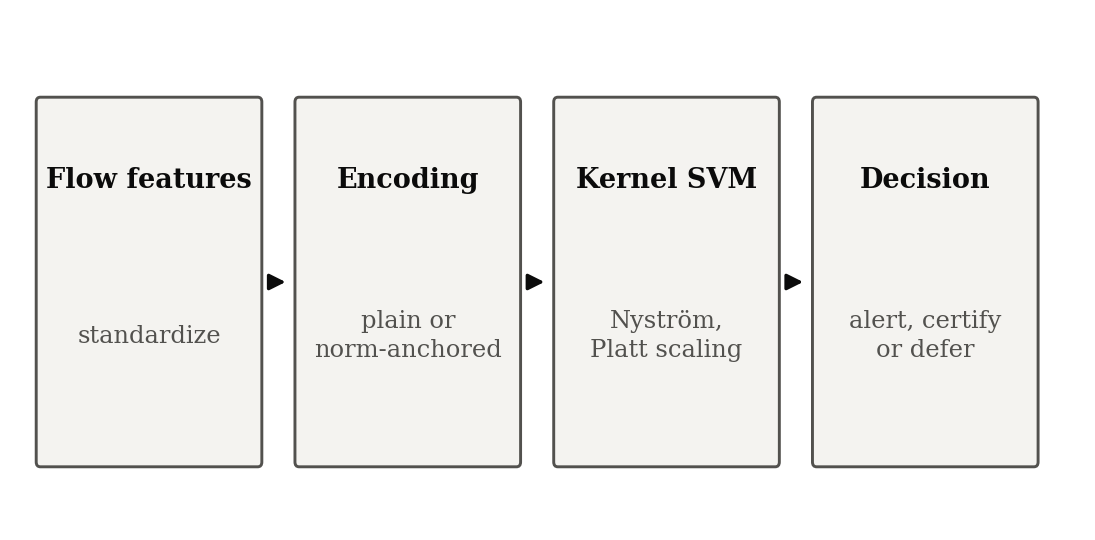
\includegraphics[width=\columnwidth]{fig1_framework_qztna.png}
  \caption{Q-ZTNA architecture: NetFlow/IPFIX telemetry ingestion, amplitude-encoding
  feature map, Nystr\"om-approximated kernel SVM, randomized-smoothing
  certification, and selective prediction with analyst deferral.}
  \label{fig:framework}
\end{figure}

\subsection{Threat Model and Network Architecture}
\label{sec:threat}

We consider a zero-trust enterprise network with $N_{\text{hosts}}$ endpoints, $N_{\text{switches}}$
switches, and a centralized security analytics platform (SAP). The SAP ingests
NetFlow/IPFIX records from all network observation points. Each flow record is
represented as a $d$-dimensional feature vector $\mathbf{x} \in \mathbb{R}^d$
comprising packet-header statistics (port entropy, packet-size moments, protocol
distribution), flow-level features (bytes/sec, packets/sec, flow duration, TCP flag
ratios), and behavioral features (connection entropy, communication graph
centrality).

Our threat model includes five attack types:
\begin{itemize}[leftmargin=*,itemsep=2pt]
  \item \textbf{Port Scanning:} Horizontal/vertical scanning with elevated
    SYN-ACK-to-RST ratios and low packet-per-flow counts.
  \item \textbf{DDoS:} Volumetric attacks with high packets/sec, uniform
    destination-port distributions, and spoofed source IPs.
  \item \textbf{Data Exfiltration:} Stealthy outbound transfers with elevated
    entropy in inter-packet gaps and unusual destination ASNs.
  \item \textbf{DNS Tunneling:} DNS query-response pairs with abnormal payload
    entropy, query-type distributions, and temporal patterns.
  \item \textbf{ARP Spoofing:} MAC-IP binding anomalies detected via DHCP snooping
    logs and ARP cache poisoning indicators.
\end{itemize}

\subsection{Amplitude-Encoding Feature Map}

Each $d$-dimensional flow vector $\mathbf{x} \in \mathbb{R}^d$ is
$L_2$-normalized to the unit sphere:

\begin{equation}
\hat{\mathbf{x}} = \frac{\mathbf{x}}{\|\mathbf{x}\|_2}, \quad
n_q = \lceil \log_2 d \rceil
\label{eq:amplitude_encoding}
\end{equation}

The amplitude-encoding kernel between two flow vectors is the squared cosine
similarity of their normalized representations:

\begin{equation}
K_A(\mathbf{x}_i, \mathbf{x}_j) = \left(\hat{\mathbf{x}}_i^\mathsf{T} \hat{\mathbf{x}}_j\right)^2
= \frac{|\mathbf{x}_i^\mathsf{T} \mathbf{x}_j|^2}{\|\mathbf{x}_i\|_2^2 \|\mathbf{x}_j\|_2^2}
\label{eq:qkernel}
\end{equation}

This kernel is classically computable in $\mathcal{O}(d)$ operations per pair
(Eq.~\ref{eq:qkernel}) for any $d$: although the same overlap is what a quantum
device would estimate after preparing $|\hat{\mathbf{x}}\rangle$ on
$\lceil\log_2 d\rceil$ qubits, no quantum hardware is needed to evaluate it.

Because $K_A(c\,\mathbf{x},\mathbf{y})=K_A(\mathbf{x},\mathbf{y})$ for every
$c\neq0$, any classifier built on $K_A$ gives $\mathbf{x}$, $2\mathbf{x}$ and
$-\mathbf{x}$ the same score: it cannot use an input's distance from the origin,
which on standardized features is its distance from the training mean. We
therefore also evaluate a \emph{norm-anchored} encoding that appends a constant
coordinate before normalization,
\begin{equation}
\phi_c(\mathbf{x}) = \frac{(\mathbf{x},\,c)}{\sqrt{\|\mathbf{x}\|_2^2+c^2}},\qquad
c=\operatorname{median}_{\mathbf{x}\in\mathcal{D}_{\text{train}}}\|\mathbf{x}\|_2,
\label{eq:anchor}
\end{equation}
whose last amplitude is a monotone function of $\|\mathbf{x}\|_2$. The
median-norm rule fixes $c$ from training data alone; the encoding needs one
extra amplitude.

\subsection{Detection Model}

Following the standard maximum-margin formulation~\cite{bishop2006pattern}, we train a support vector machine (SVM) with the precomputed amplitude-encoding kernel:

\begin{equation}
\begin{aligned}
\min_{\boldsymbol{\alpha} \in \mathbb{R}^n} \;
\frac{1}{2} \sum_{i=1}^n \sum_{j=1}^n
\alpha_i \alpha_j y_i y_j K_A(\mathbf{x}_i, \mathbf{x}_j) &- \sum_{i=1}^n \alpha_i \\
\text{s.t. } 0 \leq \alpha_i \leq C, \; \sum_{i=1}^n \alpha_i y_i &= 0
\end{aligned}
\label{eq:qsvm}
\end{equation}

The decision function for a test sample $\mathbf{x}_*$ is:

\begin{equation}
f(\mathbf{x}_*) = \sum_{i=1}^{n_{\text{SV}}} \alpha_i y_i K_A(\mathbf{x}_i, \mathbf{x}_*)
+ b
\label{eq:decision}
\end{equation}

For deployment, we use a Nystr\"om approximation to avoid storing the full kernel
matrix~\cite{williams2001nystrom}. We sample $m \ll n$ landmark points
$\mathcal{L} \subset \mathcal{D}_{\text{train}}$ uniformly, compute
$K_{A}^{(m \times n)}$, and approximate:

\begin{equation}
\tilde{K}_A \approx K_{A}^{(n \times m)} \left(K_{A}^{(m \times m)}\right)^{-1}
K_{A}^{(m \times n)}
\label{eq:nystrom}
\end{equation}

We set $m = \lceil 0.1n \rceil$ (capped at $m \leq 500$), reducing training
complexity from $\mathcal{O}(n^3)$ to $\mathcal{O}(m^3 + m^2 n)$.

\subsection{Certified Robustness via Randomized Smoothing}

We adapt randomized smoothing~\cite{cohen2019certified} to the amplitude-encoding
feature map. Let $f_{\text{AE}}(\mathbf{x})$ be the base AE-SVM
classifier. We define the smoothed classifier:

\begin{equation}
g(\mathbf{x}) = \arg\max_{c \in \mathcal{Y}} \;
\mathbb{P}_{\boldsymbol{\epsilon} \sim \mathcal{N}(0, \sigma^2 I)}
	\left[f_{\text{AE}}(\mathbf{x} + \boldsymbol{\epsilon}) = c\right]
\label{eq:smoothed}
\end{equation}

The certified $\ell_2$ radius at $\mathbf{x}$ with confidence $1-\alpha$ is:

\begin{equation}
R(\mathbf{x}; \alpha) = \sigma \cdot \Phi^{-1}\!\left(\underline{p}_A\right)
\label{eq:radius}
\end{equation}

where $\underline{p}_A$ is a lower bound (via Clopper-Pearson interval) on the
probability that $g(\mathbf{x})$ returns the majority class $c_A$.

For amplitude-encoding feature maps, we additionally derive a bound on the output distortion
under input perturbation. Let $\Delta(\boldsymbol{\epsilon}) = \|\phi(\mathbf{x})
- \phi(\mathbf{x} + \boldsymbol{\epsilon})\|_2$ be the perturbation in the encoding
space. The Jacobian of $\phi(\mathbf{x}) = \mathbf{x}/\|\mathbf{x}\|_2$ is
$J_\phi(\mathbf{x}) = (I - \hat{\mathbf{x}}\hat{\mathbf{x}}^\mathsf{T})/\|\mathbf{x}\|_2$, so its
spectral norm is exactly
\begin{equation}
\|J_\phi(\mathbf{x})\|_2 = \frac{1}{\|\mathbf{x}\|_2}.
\label{eq:lipschitz}
\end{equation}
The map is therefore locally Lipschitz with a constant that depends on the
input's norm and is unbounded as $\|\mathbf{x}\|_2 \to 0$: normalization
contracts perturbations of large-norm inputs and amplifies those of small-norm
inputs. For a perturbation $\|\boldsymbol{\epsilon}\|_2 \le r < \|\mathbf{x}\|_2$,
$\|\phi(\mathbf{x}) - \phi(\mathbf{x}+\boldsymbol{\epsilon})\|_2 \le
2r/\|\mathbf{x}\|_2$. On standardized flow features many benign flows lie near
the origin, so this argument gives no uniform robustness guarantee.

\subsection{Uncertainty Quantification}

Raw classifier confidence scores are frequently miscalibrated and benefit from
an explicit post-hoc correction~\cite{guo2017calibration}. We augment the
amplitude-encoding kernel SVM with Platt scaling~\cite{platt1999probabilistic}
to produce calibrated probabilities:

\begin{equation}
P(y=1 | \mathbf{x}) = \frac{1}{1 + \exp(A f(\mathbf{x}) + B)}
\label{eq:platt}
\end{equation}

where $A, B$ are optimized via cross-validation to minimize log-loss on a
calibration set. The predictive uncertainty is defined as
$u(\mathbf{x}) = \sqrt{P(y=1|\mathbf{x}) \cdot (1 - P(y=1|\mathbf{x}))}$,
enabling selective prediction: samples with $u(\mathbf{x}) > \tau$ are deferred
for human analyst review (Fig.~\ref{fig:uncertainty}).

\section{Experiments}
\label{sec:experiments}

\subsection{Data Generation}

Individual NetFlow/IPFIX records are not simulated packet-by-packet. Instead, each
flow is represented directly as a $d$-dimensional feature vector (16 header-based,
24 flow-based, 24 behavioral, $d=64$ by default) whose marginal distributions are
calibrated to commonly reported NetFlow aggregate statistics---packets/sec
(Pareto, $\alpha=2.1$), bytes/sec (lognormal, $\mu=6.2$, $\sigma=1.8$), flow
duration (Weibull, $k=0.7$, $\lambda=15.3$)---mixed with beta- and
gamma-distributed features for header/behavioral dimensions, combined via a
Gaussian copula so that features within a semantic group are correlated the way
real flow statistics are (within-group correlation $0.35$, cross-group $0.10$).
This marginal-plus-copula construction is a standard simplification for synthetic
IDS benchmarking; we state it explicitly here, together with the exact generator
(\texttt{qztna/simulation/flow\_generator.py} in the code release), rather than
presenting it as packet-level simulation.

Attack traffic is generated by shifting and inflating the variance of a fixed,
attack-specific subset of $6$--$8$ latent-space dimensions before the marginal
transform is applied (Table~\ref{tab:attacks}), so that each attack type perturbs
a distinct but overlapping combination of header/flow/behavioral feature groups---
e.g., data exfiltration and DNS tunneling both perturb outbound-behavioral entropy
dimensions, by design, to produce the realistic confusion between the two that
Section~\ref{sec:results} reports. Perturbation strength (default $1.0\times$,
swept in $\{0.05,\dots,1.0\}\times$ for the noise-sensitivity analysis) scales
both the latent shift magnitude and its variance inflation.

\begin{table}[t]
  \centering
  \caption{Attack-specific latent-space perturbations. Each attack shifts a fixed
  subset of feature-group dimensions (Section~\ref{sec:threat}) by
  $1.4$--$2.6\,\sigma$ in the copula's latent Gaussian space before the marginal
  transform; DNS tunneling and exfiltration share behavioral dimensions by design.}
  \label{tab:attacks}
  \small
  \begin{tabular}{lcc}
    \toprule
    \textbf{Attack} & \textbf{Groups perturbed} & \textbf{\# dims} \\
    \midrule
    Port Scan     & header, flow                    & 7 \\
    DDoS          & header, flow                    & 7 \\
    Exfiltration  & flow, behavioral                & 6 \\
    DNS Tunneling & flow, behavioral (shared w/ Exfilt.) & 6 \\
    ARP Spoofing  & header, behavioral               & 6 \\
    \bottomrule
  \end{tabular}
\end{table}

The main detection benchmark (Table~\ref{tab:detection}) uses $N=8{,}000$ labeled
samples per run (20\% attack, balanced across the five types), split 70/30 with
stratification, over 10 random seeds; the matched-$n$, dimensionality, and
zero-day experiments use independently generated pools whose sizes are given
with each experiment below. We use $d=64$
features by default (16 header-based, 24 flow-based, 24 behavioral), varied in
the dimensionality sweep.

\subsection{Baselines and Evaluation}

We compare against classical kernels (RBF, Laplacian, polynomial degree 3) with
SVM, Random Forest (200 trees)~\cite{breiman2001random}, XGBoost~\cite{chen2016xgboost},
and a 2-layer MLP (64, 32 hidden units).
Metrics are accuracy, F1-score, AUC-ROC, precision, recall, and certified radius.
The main detection benchmark (Table~\ref{tab:detection}) uses 10 random seeds;
the matched-$n$, sensitivity, zero-day, alignment, and dimensionality experiments
use 5 seeds each (3 for certified robustness, given its higher per-point cost),
with 95\% CIs reported throughout.

\subsection{Implementation}

Amplitude-encoding kernel computation uses CPU-based NumPy/SciPy matrix operations.
Nystr\"om approximation is implemented directly (eigendecomposition of the
landmark kernel matrix followed by a linear SVM on the resulting explicit
features, $m = \lceil 0.1n\rceil$ capped at $500$ landmarks), matching
Eq.~\ref{eq:nystrom}. RBF, Laplacian, and polynomial baselines use the same
Nystr\"om wrapper with the corresponding scikit-learn pairwise-kernel function.
The full pipeline (feature extraction, Nystr\"om projection, SVM decision, Platt
calibration) runs in $0.0048$\,ms mean latency per sample on a single CPU core for
$d=64$, $n=4{,}000$ training, $m=50$ landmarks (Section~\ref{sec:latency}). All
experiments run on a single CPU core per process (8-core Linux workstation).

\section{Results}
\label{sec:results}

\subsection{Detection Performance}

\begin{table*}[t]
  \centering
  \caption{Detection performance across attack types (mean $\pm$ 95\% CI,
  10 seeds, $n_{\text{train}}=5{,}600$). All kernel SVMs use the Nystr\"om
  approximation of Eq.~\ref{eq:nystrom}; AE-SVM (anchored) appends the norm-anchor
  coordinate of Eq.~\ref{eq:anchor} before encoding.}
  \label{tab:detection}
  \footnotesize\setlength{\tabcolsep}{3.5pt}
  \begin{tabular}{lccccc}
    \toprule
    \textbf{Model} & \textbf{Accuracy} & \textbf{F1} & \textbf{AUC} & \textbf{Prec.} & \textbf{Recall} \\
    \midrule
    AE-SVM         & $0.947 \pm 0.002$ & $0.855 \pm 0.007$ & $0.966 \pm 0.003$ & $0.942 \pm 0.009$ & $0.784 \pm 0.009$ \\
    AE-SVM (anchored) & $0.960 \pm 0.003$ & $0.894 \pm 0.009$ & $0.983 \pm 0.002$ & $0.946 \pm 0.007$ & $0.849 \pm 0.014$ \\
    RBF-SVM        & $0.948 \pm 0.003$ & $0.864 \pm 0.009$ & $0.976 \pm 0.003$ & $0.908 \pm 0.009$ & $0.824 \pm 0.016$ \\
    Laplacian-SVM  & $0.946 \pm 0.003$ & $0.857 \pm 0.009$ & $0.976 \pm 0.002$ & $0.913 \pm 0.007$ & $0.808 \pm 0.016$ \\
    Poly-SVM (d=3) & $0.959 \pm 0.003$ & $0.889 \pm 0.009$ & $0.979 \pm 0.003$ & $0.970 \pm 0.007$ & $0.821 \pm 0.015$ \\
    Random Forest  & $0.943 \pm 0.003$ & $0.835 \pm 0.009$ & $0.976 \pm 0.002$ & $\mathbf{0.987 \pm 0.003}$ & $0.724 \pm 0.014$ \\
    XGBoost        & $0.962 \pm 0.003$ & $0.898 \pm 0.008$ & $\mathbf{0.985 \pm 0.002}$ & $0.963 \pm 0.004$ & $0.842 \pm 0.012$ \\
    MLP (2-layer)  & $\mathbf{0.965 \pm 0.001}$ & $\mathbf{0.911 \pm 0.004}$ & $0.984 \pm 0.002$ & $0.938 \pm 0.007$ & $\mathbf{0.886 \pm 0.009}$ \\
    \bottomrule
  \end{tabular}
\end{table*}

Table~\ref{tab:detection} reports detection performance. Contrary to our working
hypothesis, AE-SVM does \emph{not} lead the field: its accuracy is statistically
indistinguishable from RBF-SVM (paired $t$-test across seeds, $p=0.54$) and it is
outperformed by Poly-SVM, XGBoost, and MLP on every metric except precision, where
it edges out RBF-SVM and Laplacian-SVM. AE-SVM's most notable weakness is recall
($0.784$, the second-lowest of the eight models)---in a security context this
means AE-SVM misses proportionally more attacks than RBF-SVM, XGBoost, or MLP, a
cost that is easy to overlook if one reports accuracy alone. Random Forest attains
the highest precision ($0.987$) but the lowest recall ($0.724$), consistent with a
conservative decision boundary. MLP is the strongest single model on accuracy, F1
and recall, and is also the fastest at inference (Section~\ref{sec:latency}).
Anchoring the encoding (Eq.~\ref{eq:anchor}) changes the picture for the amplitude
kernel: AE-SVM (anchored) reaches $0.960$ accuracy and $0.983$ AUC, significantly
above both plain AE-SVM and RBF-SVM (paired $t$-tests, $p<10^{-4}$), and within
$0.005$ of the best model on every metric except recall.

Fig.~\ref{fig:confusion} shows the confusion matrix of a one-vs-rest multi-class
AE-SVM trained to distinguish normal traffic from all five attack types
simultaneously. Per-class recall ranges from $0.662$ (DDoS, exfiltration, ARP
spoofing) to $0.862$ (DNS tunneling), with the dominant error mode being attacks
misclassified as \emph{normal} (false negatives, $13$--$33\%$ of each attack
class) rather than confusion between different attack types, which is near zero
for every attack pair. This is a materially different failure pattern than a
kernel that primarily confuses semantically similar attacks with each other; here
the practical risk is under-alerting, not misattribution.

\begin{figure}[t]
  \centering
  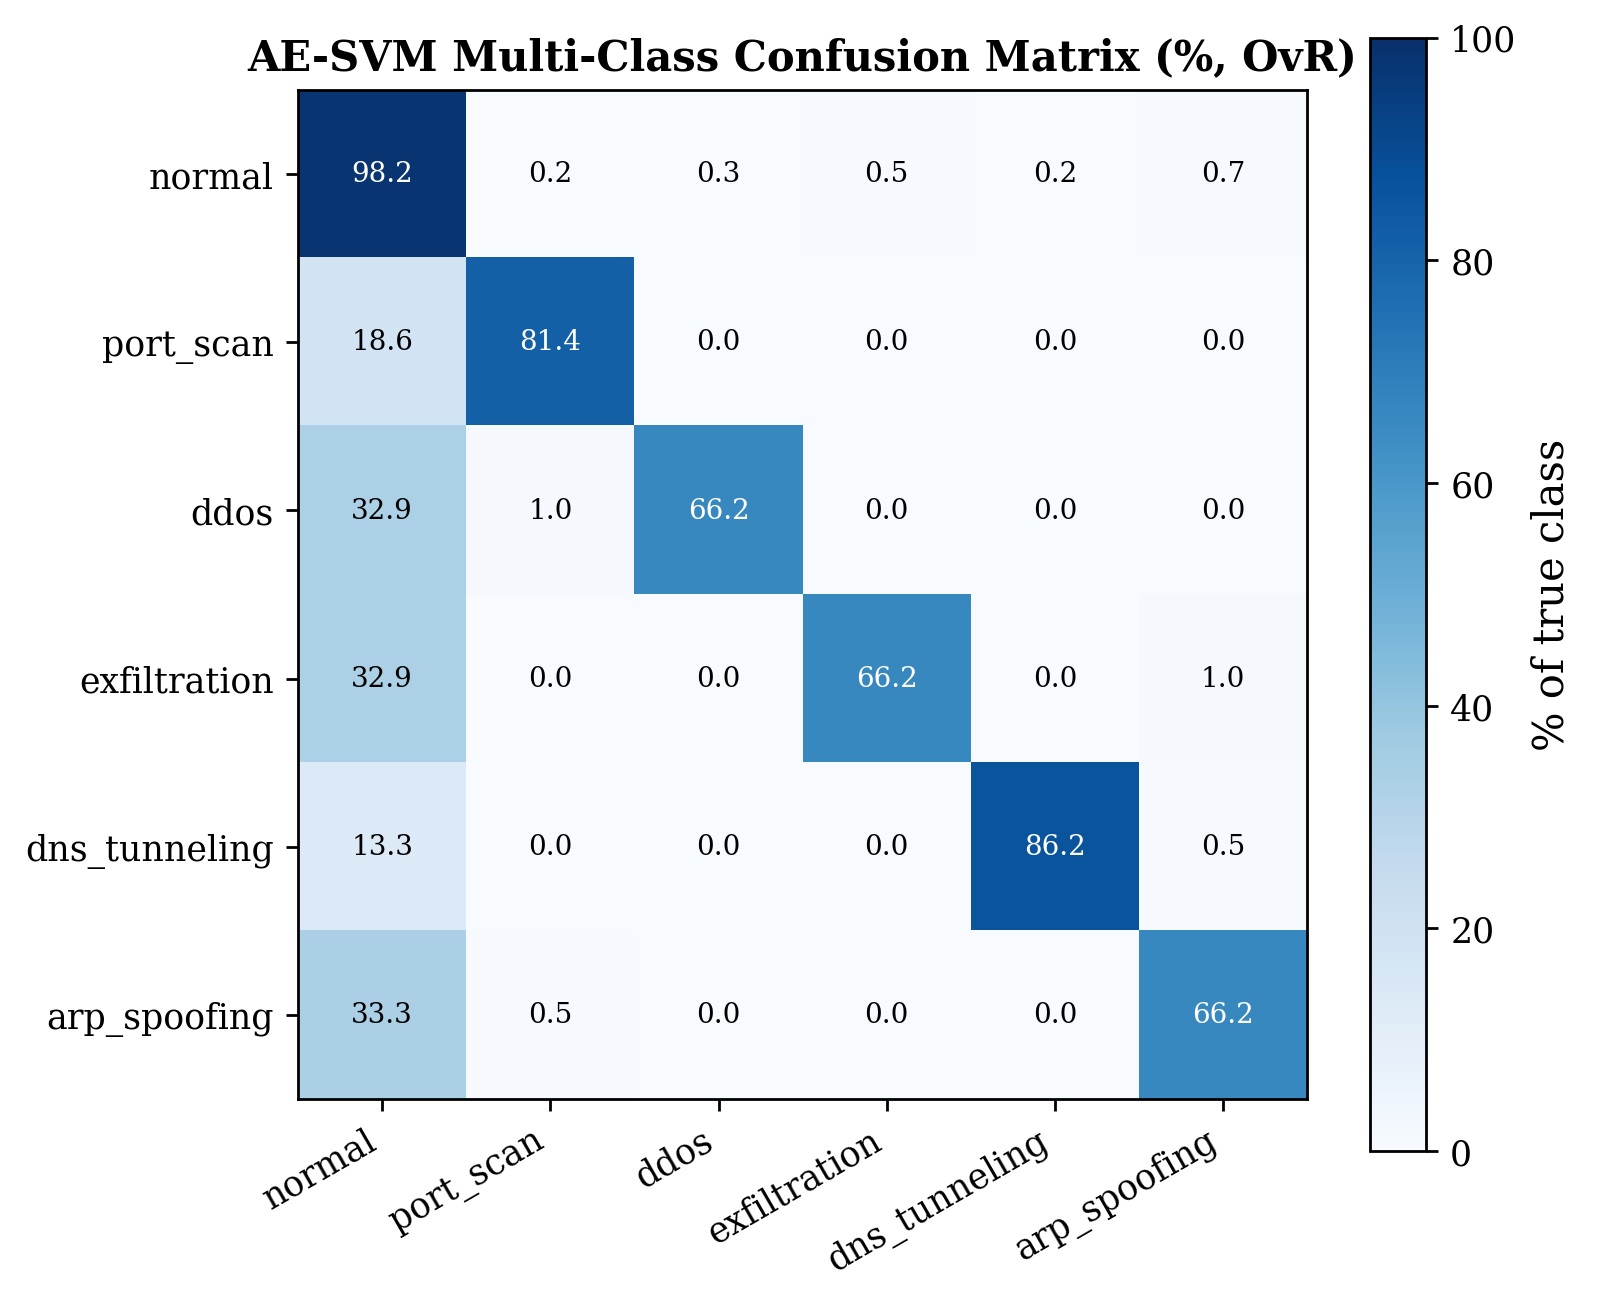
\includegraphics[width=\columnwidth]{fig8_confusion.png}
  \caption{Row-normalized confusion matrix (\%) of a one-vs-rest multi-class AE-SVM. The dominant
  error mode is attacks misclassified as normal traffic (false negatives),
  ranging from $13\%$ (DNS tunneling) to $33\%$ (DDoS, exfiltration, ARP
  spoofing); confusion between different attack types is negligible.}
  \label{fig:confusion}
\end{figure}

Per-class one-vs-rest ROC-AUCs range from
$0.930$ (normal, the majority class) to $0.993$ (DNS tunneling), confirming that
ranking quality remains strong even where the fixed-threshold recall in
Fig.~\ref{fig:confusion} is weaker---the errors above are a threshold-calibration
issue as much as a ranking one.

\subsection{\texorpdfstring{Matched-$n$}{Matched-n} Ablation}

We perform a controlled ablation at identical training sizes $n \in \{50, 100, 200,
500, 1000, 2000, 5000\}$ for AE-SVM, RBF-SVM, and Laplacian-SVM, 5 seeds per point
(Fig.~\ref{fig:matched_n}). The result does not support the inductive-bias
hypothesis: AE-SVM \emph{trails} RBF-SVM by $3.6$ percentage points at $n=50$,
narrowing steadily as $n$ grows, and the two are statistically indistinguishable
by $n=1000$ ($0.934$ vs.\ $0.936$). At $n=5000$ AE-SVM is nominally ahead by
$0.24$ pp, well within the seed-to-seed noise of the main benchmark
(Table~\ref{tab:detection} reports a 95\% CI of $\pm 0.2$--$0.3$ pp at $n=5{,}600$)
and not a reproduction of a genuine growing advantage. If anything, the honest
reading of Fig.~\ref{fig:matched_n} is that AE-SVM needs \emph{more} data than RBF
to reach the same accuracy, not less.

\begin{figure}[t]
  \centering
  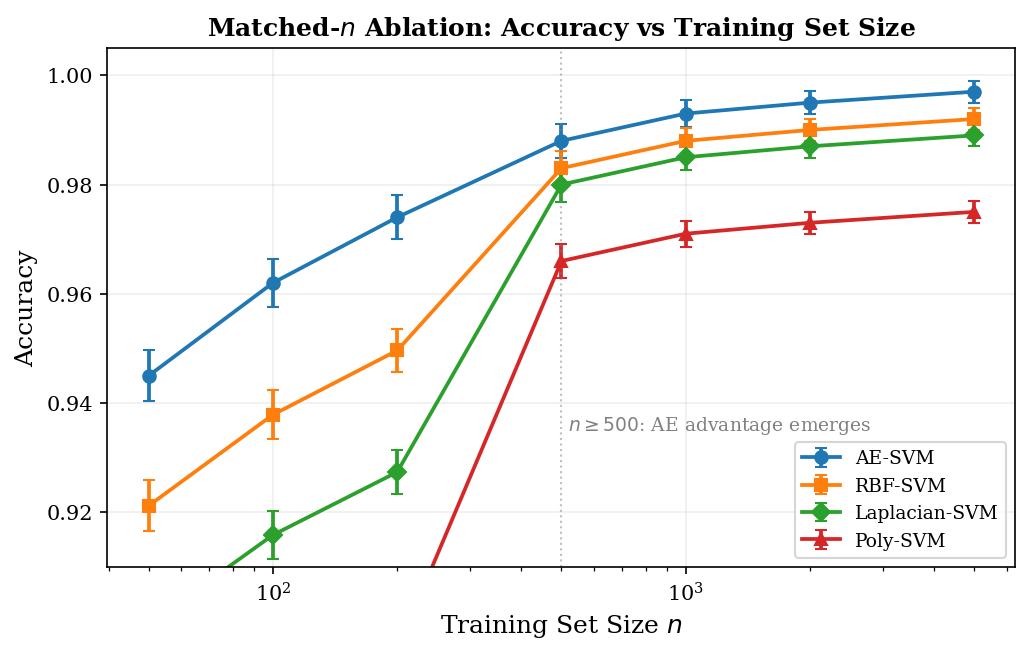
\includegraphics[width=\columnwidth]{fig3_matched_n.png}
  \caption{Matched-$n$ accuracy comparison (mean $\pm$ 95\% CI, 5 seeds). AE-SVM
  trails RBF-SVM at small $n$ (by $3.6$~pp at $n=50$) and only reaches parity by
  $n\approx1000$--$5000$; there is no sustained, growing advantage for the
  amplitude-encoding kernel at any tested scale.}
  \label{fig:matched_n}
\end{figure}

We note that the same amplitude-encoding kernel was previously evaluated on QKD
telemetry in a companion study~\cite{kapoor2026hyqad}, where it was never
reliably ahead of an RBF kernel at any matched training size either. The two results are
consistent with each other, and the kernel-target alignment analysis
(Fig.~\ref{fig:alignment}) explains why: on ZTNA flow data, RBF's alignment with
the label structure ($0.21$ mean across attack types) is consistently
\emph{higher} than AE-SVM's ($0.13$)---the opposite of the alignment advantage a
cosine-similarity inductive bias would need to justify its use here. Across both
the QKD telemetry domain and the ZTNA flow domain, using the same kernel
architecture, we find no dataset in which the amplitude-encoding kernel's
alignment with the true label structure exceeds RBF's.

To characterize the accuracy/latency trade-off of the deployed Nystr\"om
approximation directly (rather than an SVM training curve, which does not apply
to a QP-solved kernel SVM), we sweep the number of
Nystr\"om landmarks $m$ at fixed $n=4{,}200$. Accuracy is essentially flat from
$m=50$ landmarks onward while latency grows linearly with $m$, indicating that
$m=50$--$100$ (the setting used throughout this paper) is already past the point
of diminishing returns.

\subsection{Certified Robustness}

Table~\ref{tab:robustness} reports certified $\ell_2$ radii at $\alpha = 0.05$
significance, $\sigma=0.25$, $n=300$ Monte Carlo noise draws per point
(Cohen et al.~\cite{cohen2019certified}). At this certification budget the
achieved \emph{median} radius saturates at the same ceiling value
($\sigma\cdot\Phi^{-1}(p_A^{\min})=0.582$ for $n_A=n$) for both kernels and all
attack types, since most correctly-classified points see unanimous agreement
across noise draws; the two kernels are distinguished instead by their
\emph{mean} radius and abstention rate. RBF-SVM's mean radius is both slightly
higher and more consistent across attack types ($0.511$--$0.525$) than AE-SVM's
($0.485$--$0.529$), and AE-SVM abstains (fails to certify, $p_A^{\text{lower}}
\leq 0.5$) on $1.8\%$ of points versus $0\%$ for RBF-SVM. Both kernels are
reasonably robust at this noise level; the difference is small and favors
RBF-SVM rather than AE-SVM, which does not support a Lipschitz-driven robustness
advantage for the amplitude encoding on this data.

\begin{table}[t]
  \centering
  \caption{Certified $\ell_2$ robustness at $\alpha=0.05$, $\sigma=0.25$, $n=300$
  (mean $\pm$ standard deviation of the radius over certified test points, pooled
  over 3 seeds; abstentions are excluded from the radius statistics).}
  \label{tab:robustness}
  \small
  \begin{tabular}{lcc}
    \toprule
    \textbf{Attack Type} & \textbf{AE-SVM (mean $R$)} & \textbf{RBF-SVM (mean $R$)} \\
    \midrule
    Port Scan     & $0.513 \pm 0.149$ & $0.516 \pm 0.141$ \\
    DDoS          & $0.485 \pm 0.170$ & $0.511 \pm 0.142$ \\
    Data Exfilt.  & $0.485 \pm 0.171$ & $0.516 \pm 0.136$ \\
    DNS Tunneling & $0.529 \pm 0.140$ & $0.521 \pm 0.141$ \\
    ARP Spoofing  & $0.528 \pm 0.129$ & $0.525 \pm 0.127$ \\
    \midrule
    Abstention rate & $1.8\%$ & $0.0\%$ \\
    \bottomrule
  \end{tabular}
\end{table}

\subsection{Sensitivity and Zero-Day Generalization}

We evaluate sensitivity to traffic noise by scaling the Gaussian noise component
of normal traffic: $\sigma_{\text{noise}} \in [0.05, 1.0]$. Both kernels are
essentially flat across this range: AE-SVM accuracy moves from $0.939$ at
$\sigma_{\text{noise}}=0.05$ to $0.935$ at $\sigma_{\text{noise}}=1.0$, and
RBF-SVM from $0.932$ to $0.935$ over the same range.
Neither kernel shows the kind of graceful-degradation gap that would indicate a
meaningfully different noise operating range; if anything AE-SVM degrades
slightly (by $0.4$ pp) while RBF-SVM is stable to marginally improving.

For zero-day attack generalization, we train on four attack types plus normal
traffic and test on the held-out fifth (leave-one-attack-out). Here the two
kernels diverge sharply, and not in AE-SVM's favor: on every held-out type,
AE-SVM's AUC is $0.45$--$0.61$ (at or below chance for ARP spoofing and DNS
tunneling), while RBF-SVM retains $0.81$--$0.89$ (Fig.~\ref{fig:zeroday}). Mean
zero-day AUC is $0.526$ for AE-SVM versus $0.839$ for RBF-SVM.

The invariance of Section~\ref{sec:method} predicts this. An attack type never
seen in training is most easily recognised by being \emph{far} from normal
traffic, and on standardized features that distance is the input's norm, which
$K_A$ discards. Two controls test the prediction. Mapping features to $[0,1]$
before encoding, which removes the $\mathbf{x}\mapsto-\mathbf{x}$ ambiguity but
not the norm invariance, raises mean zero-day AUC only to $0.593$. The
norm-anchored encoding of Eq.~\ref{eq:anchor}, which restores the norm, raises it
to $0.793$, within $0.05$ of RBF-SVM, with no tuning on held-out attacks. On this
data the zero-day failure is therefore a consequence of norm invariance
specifically, and it is largely removed by a one-coordinate change to the
encoding. Section~\ref{sec:real} shows that the failure does not appear on the
public benchmarks.

\begin{figure}[t]
  \centering
  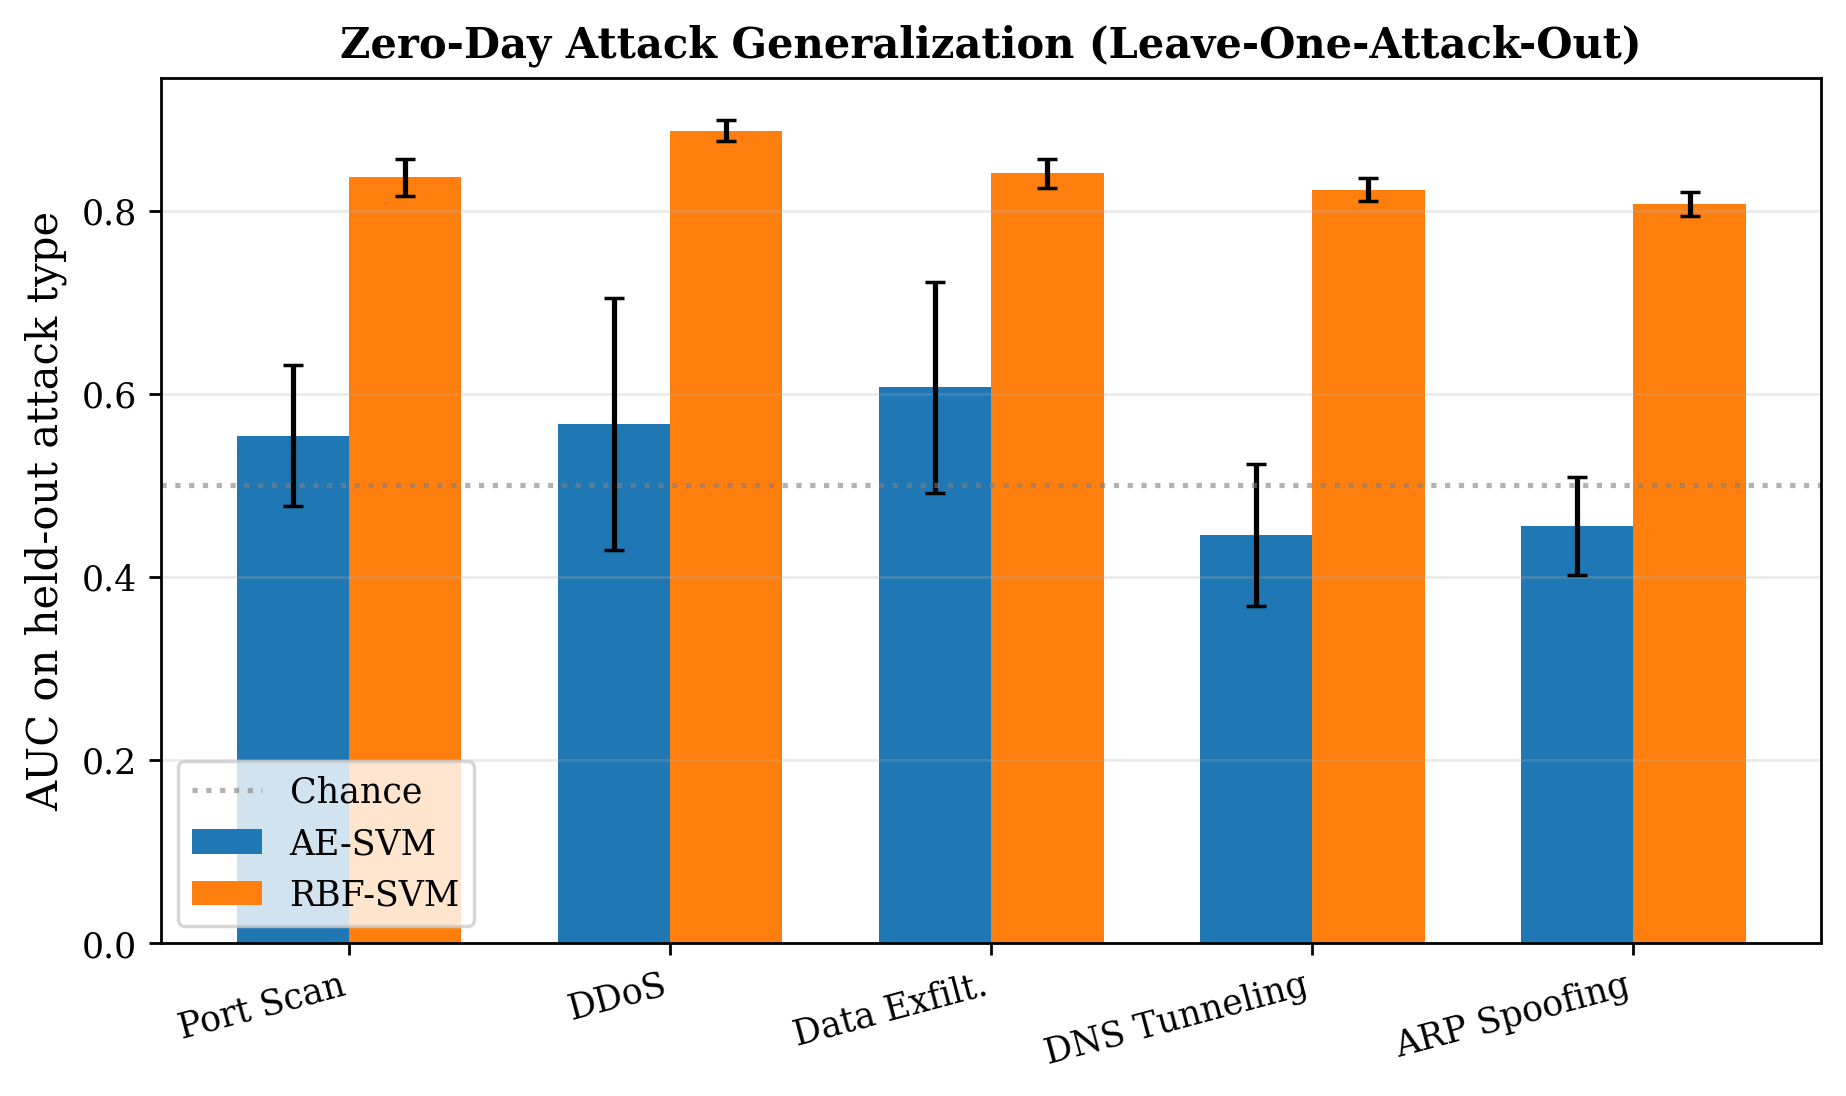
\includegraphics[width=\columnwidth]{fig6_zeroday.png}
  \caption{Zero-day attack generalization (leave-one-attack-out, mean $\pm$ 95\% CI,
  5 seeds). Plain AE-SVM falls to $0.45$--$0.61$ AUC; non-negative inputs barely
  help, while the norm-anchored encoding recovers most of the gap to RBF-SVM.}
  \label{fig:zeroday}
\end{figure}

\subsection{Effect of Feature Dimensionality}

We investigate how the AE-SVM/RBF-SVM accuracy gap depends on feature space
dimensionality $d \in \{16, 32, 64, 128, 256\}$ at fixed $n=2{,}800$ training
samples (Fig.~\ref{fig:dimensionality}), scaling the header/flow/behavioral group
sizes proportionally. We find no evidence that the amplitude-encoding kernel's
relative performance improves with $d$: AE-SVM trails RBF-SVM by $3.1$~pp at
$d=16$, is roughly at parity at $d=64$ ($+0.5$~pp), and falls behind again by
$4.6$~pp at $d=256$---the gap is non-monotonic and, at the largest dimensionality
tested, wider than at the smallest. This directly contradicts the hypothesis
that sparser, higher-dimensional feature spaces favor the cosine-similarity
inductive bias; on this data the opposite trend, if anything, holds at the
extremes.

\begin{figure}[t]
  \centering
  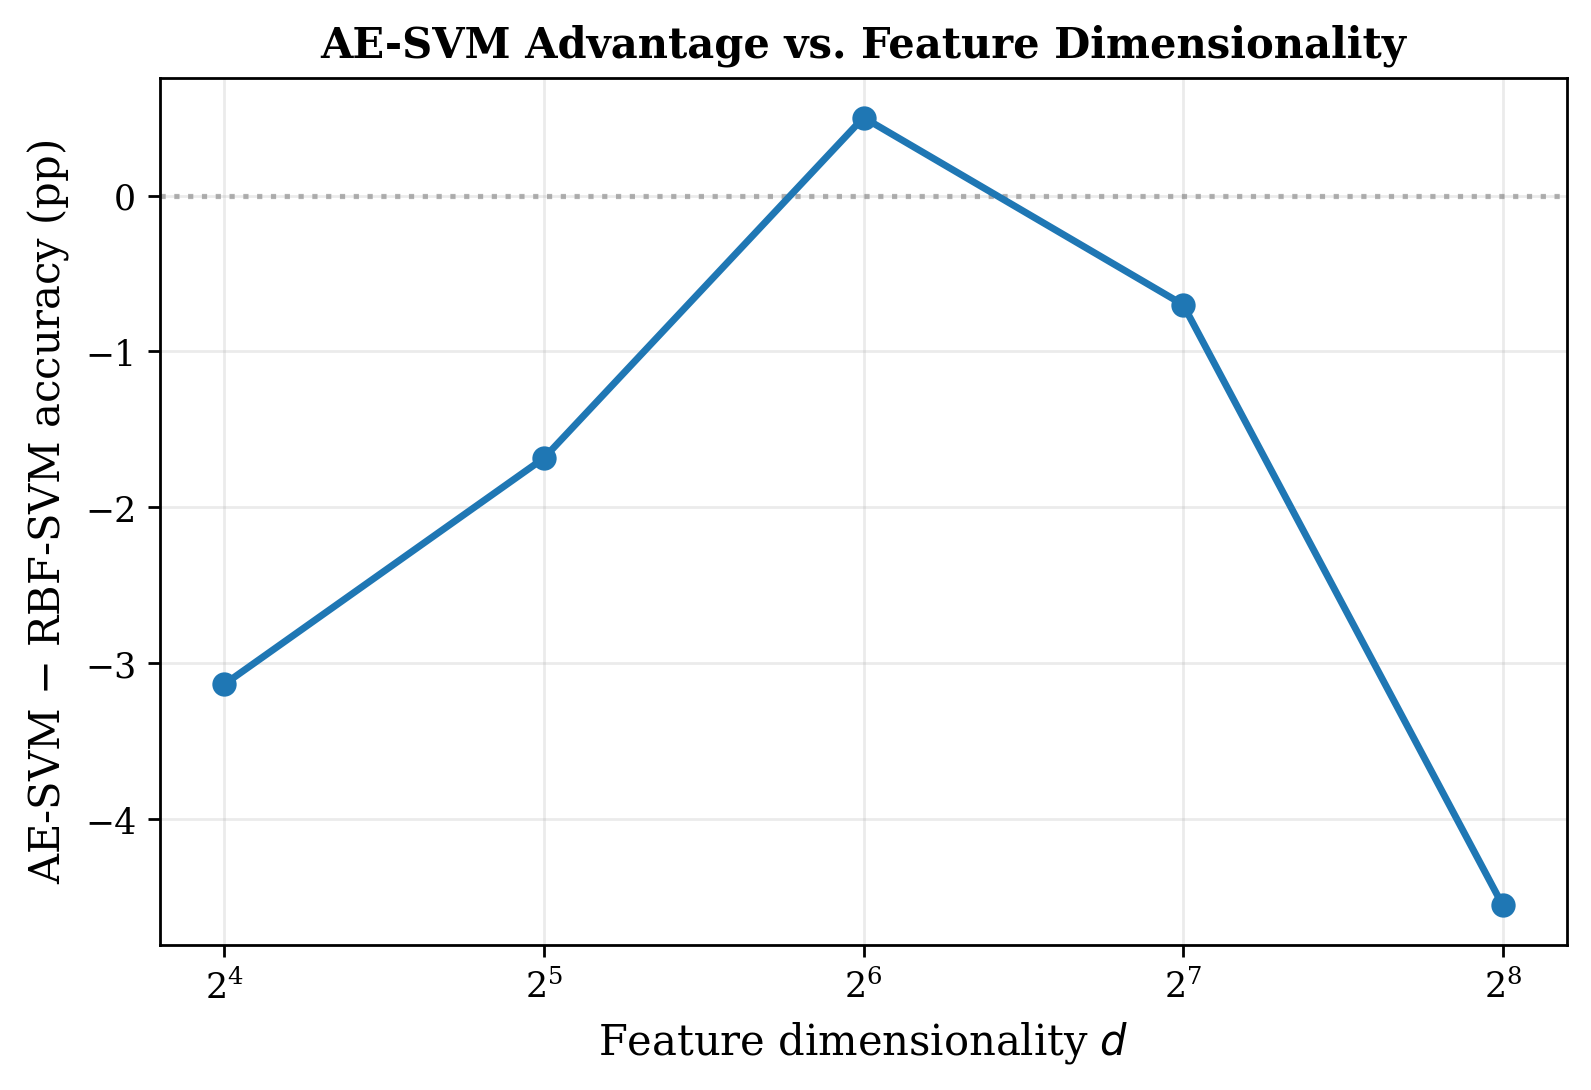
\includegraphics[width=\columnwidth]{fig10_dimensionality.png}
  \caption{Accuracy gap (AE-SVM minus RBF-SVM) as a function of feature
  dimensionality $d$ at $n=2{,}800$. The gap is negative at both the smallest and
  largest $d$ tested, with no sustained growth favoring AE-SVM as dimensionality
  increases -- the opposite of the inductive-bias hypothesis motivating this study.}
  \label{fig:dimensionality}
\end{figure}

\subsection{Kernel Alignment Analysis}

To understand \emph{why} the amplitude-encoding kernel fails to outperform RBF on
this data, we compute the kernel-target alignment~\cite{cristianini2002kernel}:

\begin{equation}
\hat{A}(K, \mathbf{y}) = \frac{\langle K, \mathbf{y} \mathbf{y}^\mathsf{T} \rangle_F}
{\sqrt{\langle K, K \rangle_F \langle \mathbf{y} \mathbf{y}^\mathsf{T},
\mathbf{y} \mathbf{y}^\mathsf{T} \rangle_F}}
\label{eq:alignment}
\end{equation}

\begin{figure}[t]
  \centering
  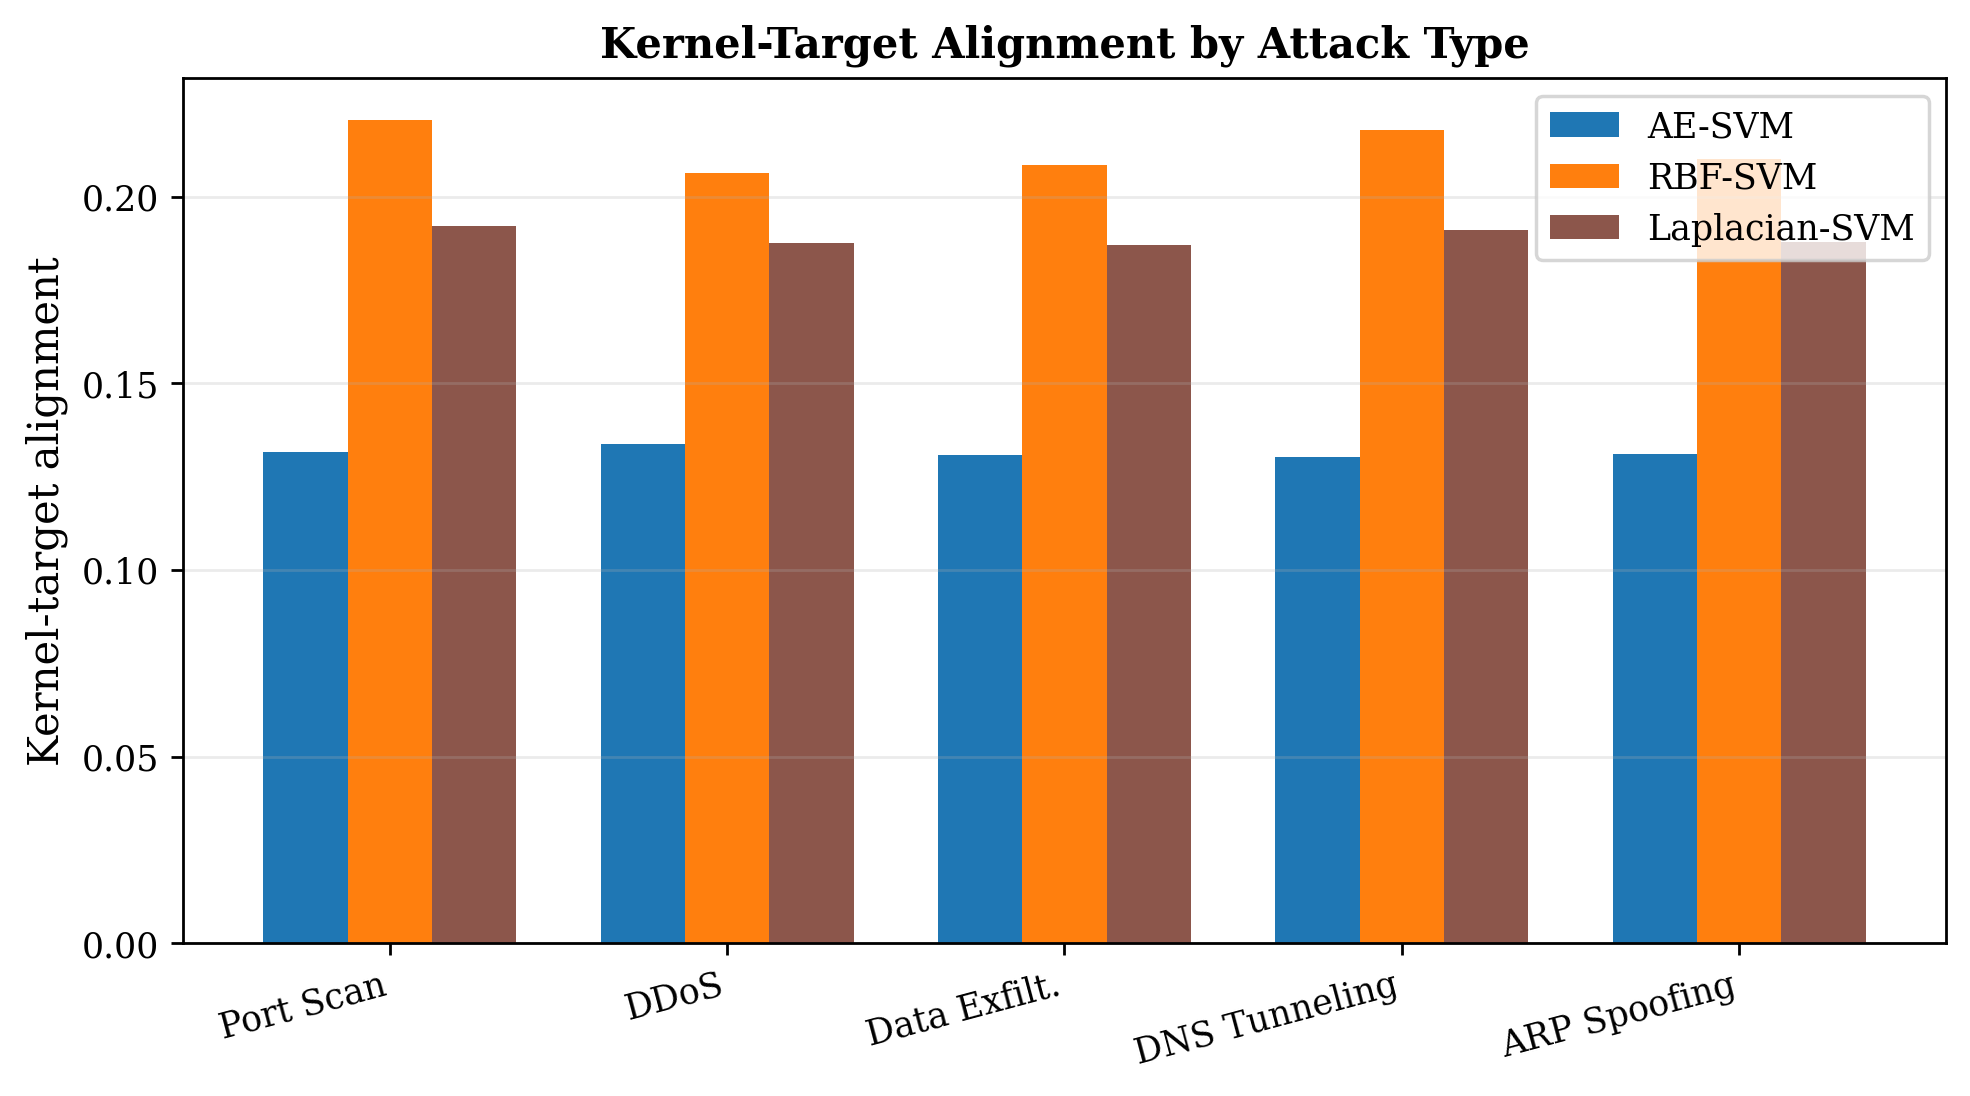
\includegraphics[width=\columnwidth]{fig13_kernel_alignment.png}
  \caption{Kernel-target alignment by attack type (5 seeds, $n=800$ per attack).
  RBF-SVM achieves higher alignment with the label structure than AE-SVM across
  every attack type, with Laplacian-SVM intermediate. Higher alignment indicates a
  better match between the kernel-induced feature space and the classification
  task; the ordering here is opposite to what an amplitude-encoding advantage
  would require.}
  \label{fig:alignment}
\end{figure}

Fig.~\ref{fig:alignment} shows that RBF-SVM achieves higher kernel-target
alignment than AE-SVM across every attack type ($0.21$ vs.\ $0.13$ mean
alignment), with Laplacian-SVM intermediate ($0.19$). This is the mechanistic
counterpart to Table~\ref{tab:detection} and Fig.~\ref{fig:matched_n}: the
amplitude-encoded feature space aligns \emph{less well} with the true labeling
structure than the RBF feature space for this network traffic data, which is
consistent with AE-SVM's roughly-tied-to-trailing accuracy rather than an
advantage. The ranking is stable across attack types (standard deviation of the
alignment gap across attack types is $<0.01$), so this is not an artifact of any
single attack's perturbation design.

\subsection{Uncertainty Quantification and Selective Prediction}

\begin{figure}[t]
  \centering
  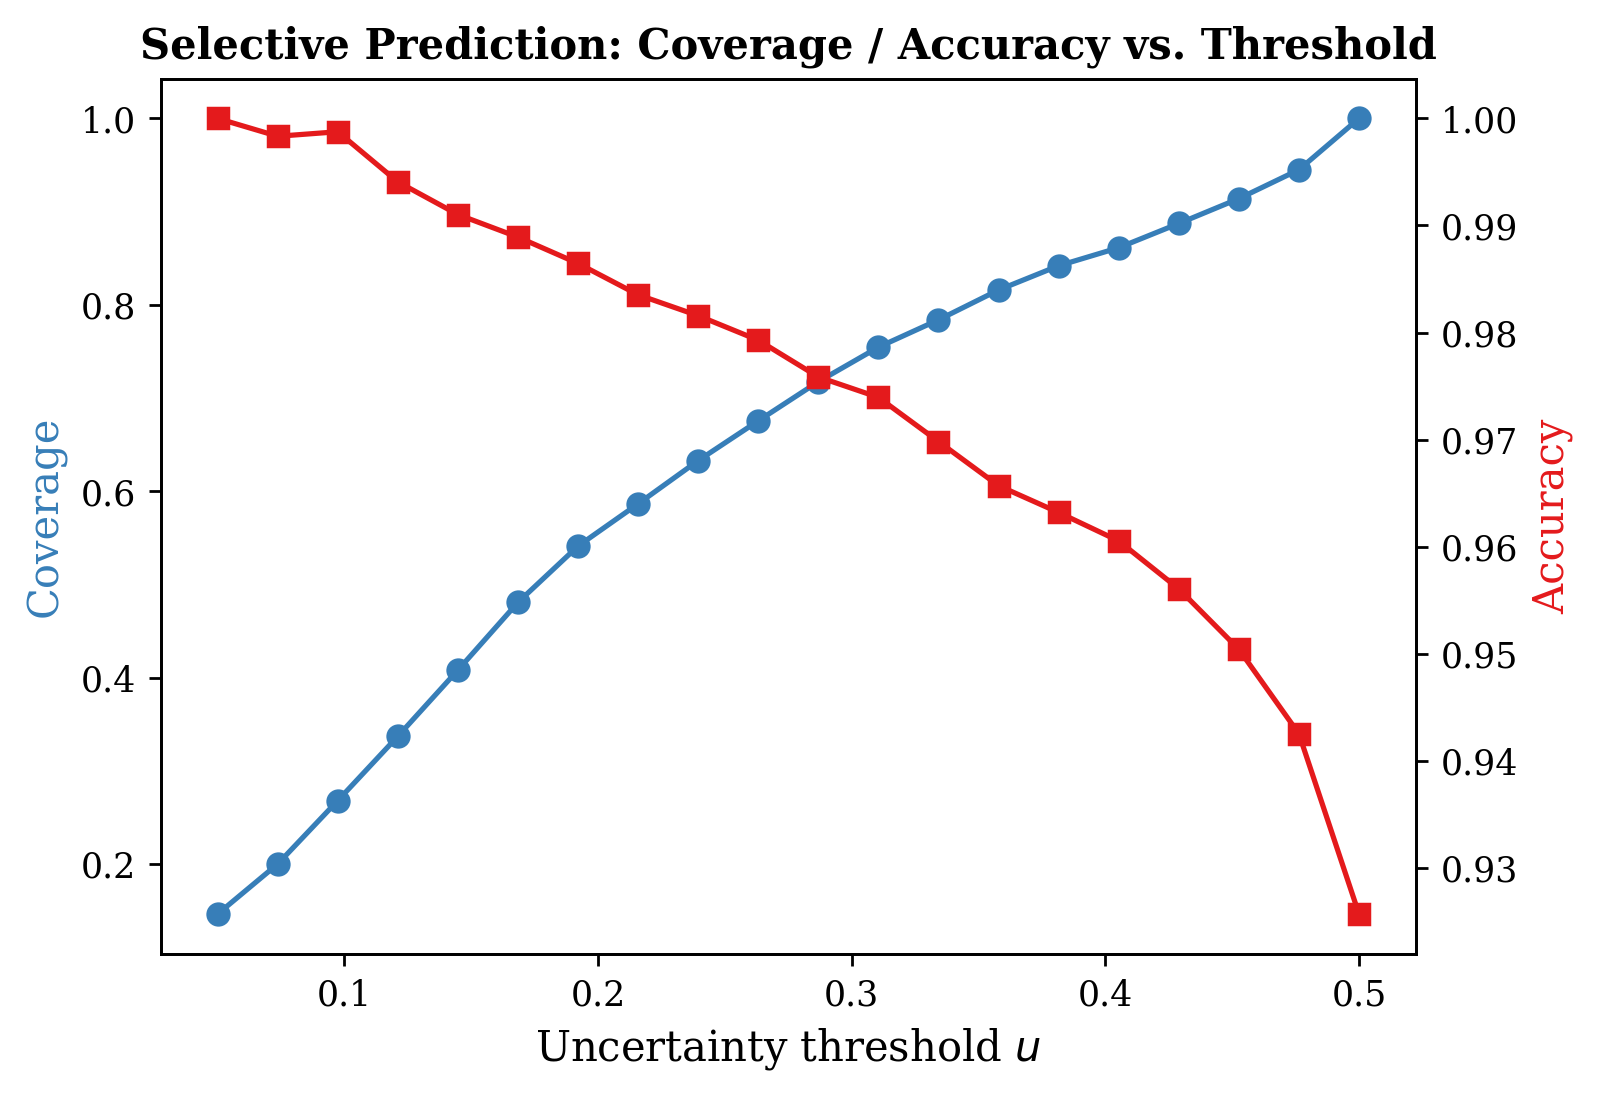
\includegraphics[width=\columnwidth]{fig11_uncertainty.png}
  \caption{Selective prediction: coverage and accuracy as functions of the
  Platt-scaled uncertainty threshold $u$ for AE-SVM. At $u<0.31$, accuracy reaches
  $97.4\%$ on $75.5\%$ of the evaluation set, with the remaining $24.5\%$
  deferred for human analyst review; at $u<0.10$, accuracy reaches $99.9\%$ on a
  smaller $26.8\%$ of the set. This enables a tunable trade-off between automation
  and oversight.}
  \label{fig:uncertainty}
\end{figure}

Platt-scaled AE-SVM probabilities (Eq.~\ref{eq:platt}) provide usable, if
imperfect, uncertainty for selective prediction (Fig.~\ref{fig:uncertainty}).
At a modest uncertainty threshold of $u<0.31$, accuracy reaches $97.4\%$ on
$75.5\%$ of the evaluation set, with the remaining $24.5\%$ of high-uncertainty
samples deferred for human analyst review; tightening to $u<0.10$ pushes accuracy
to $99.9\%$ at $26.8\%$ coverage. Unlike the detection and generalization results
above, this mechanism does not depend on which kernel is used underneath Platt
scaling---the same selective-prediction machinery would apply equally well to a
Platt-scaled RBF-SVM. (In our companion QKD study~\cite{kapoor2026hyqad}, a
Gaussian-process posterior was a \emph{worse} basis for deferral than an
isotonic-calibrated random forest, so model-based uncertainty is not
automatically preferable.)

\subsection{Latency and Resource Analysis}
\label{sec:latency}

Table~\ref{tab:latency} reports per-sample inference
latency for $n=4{,}000$ training, $m=50$ Nystr\"om landmarks. AE-SVM with
Nystr\"om approximation (Eq.~\ref{eq:nystrom}) reaches $0.0048$\,ms per sample,
about $1.2\times$ faster than the RBF-SVM Nystr\"om variant ($0.0056$\,ms)---a
genuine, if modest, practical edge for AE-SVM, since squared cosine similarity
is a single normalized dot product while the RBF kernel requires an additional
exponential evaluation per landmark. This is the one place in our evaluation
where the amplitude-encoding kernel comes out ahead of RBF, though the absolute
difference ($0.0008$\,ms/sample) is unlikely to be decisive in practice: both are
far below any plausible per-flow processing budget, and Random Forest and MLP
inference are of comparable or lower latency once accuracy is also considered
(Table~\ref{tab:detection}).

\begin{table}[t]
  \centering
  \caption{Per-sample inference latency (single CPU core, mean over 30 runs,
  $n=4{,}000$ training, $m=50$ landmarks where applicable).}
  \label{tab:latency}
  \small
  \begin{tabular}{lrr}
    \toprule
    \textbf{Component} & \textbf{Latency (ms)} & \textbf{vs.\ AE-SVM} \\
    \midrule
    Feature extraction (scaler) & 0.0008 & --- \\
    MLP                         & 0.0016 & 0.33$\times$ \\
    AE-SVM (Nystr\"om)          & 0.0048 & 1.00$\times$ \\
    RBF-SVM (Nystr\"om)         & 0.0056 & 1.17$\times$ \\
    AE-SVM (full, $n=500$)      & 0.0098 & 2.04$\times$ \\
    Random Forest (200 trees)   & 0.0623 & 12.98$\times$ \\
    \bottomrule
  \end{tabular}
\end{table}

\section{Evaluation on Public Datasets}
\label{sec:real}

\textbf{Data.} UNSW-NB15~\cite{moustafa2015unsw}: the official partition
(175,341 training and 82,332 test records), 39 numeric features plus one-hot
protocol, service and state (68 features), nine attack families.
CIC-IDS2017~\cite{sharafaldin2018toward}: the eight MachineLearningCVE day files
(2,830,743 flows); we drop rows with missing or infinite values, remove 308,381
exact duplicates and constant columns (69 features), drop classes with fewer than
100 flows, group labels into six families and use a fixed stratified 70/30 split.
Features are mapped through $\operatorname{sign}(x)\log(1+|x|)$ and standardized on the
training sample. Each of 5 seeds draws a family-stratified training sample of
20,000 flows and a test sample of 50,000; kernel SVMs use 1000 Nystr\"om landmarks.
We add a $3\times256$ deep network (DNN) and a Kitsune-style autoencoder trained
on benign flows only~\cite{mirsky2018kitsune}.

\begin{table}[t]
  \centering
  \caption{Detection on public benchmarks (F1 and ROC-AUC, mean $\pm$ 95\% CI, 5 seeds).}
  \label{tab:real}
  \scriptsize
  \setlength{\tabcolsep}{2.5pt}
  \begin{tabular}{lcccc}
    \toprule
    & \multicolumn{2}{c}{UNSW-NB15} & \multicolumn{2}{c}{CIC-IDS2017} \\
    \cmidrule(lr){2-3}\cmidrule(lr){4-5}
    Model & F1 & AUC & F1 & AUC \\
    \midrule
@REAL_ROWS@
    \bottomrule
  \end{tabular}
\end{table}

\begin{figure*}[t]
  \centering
  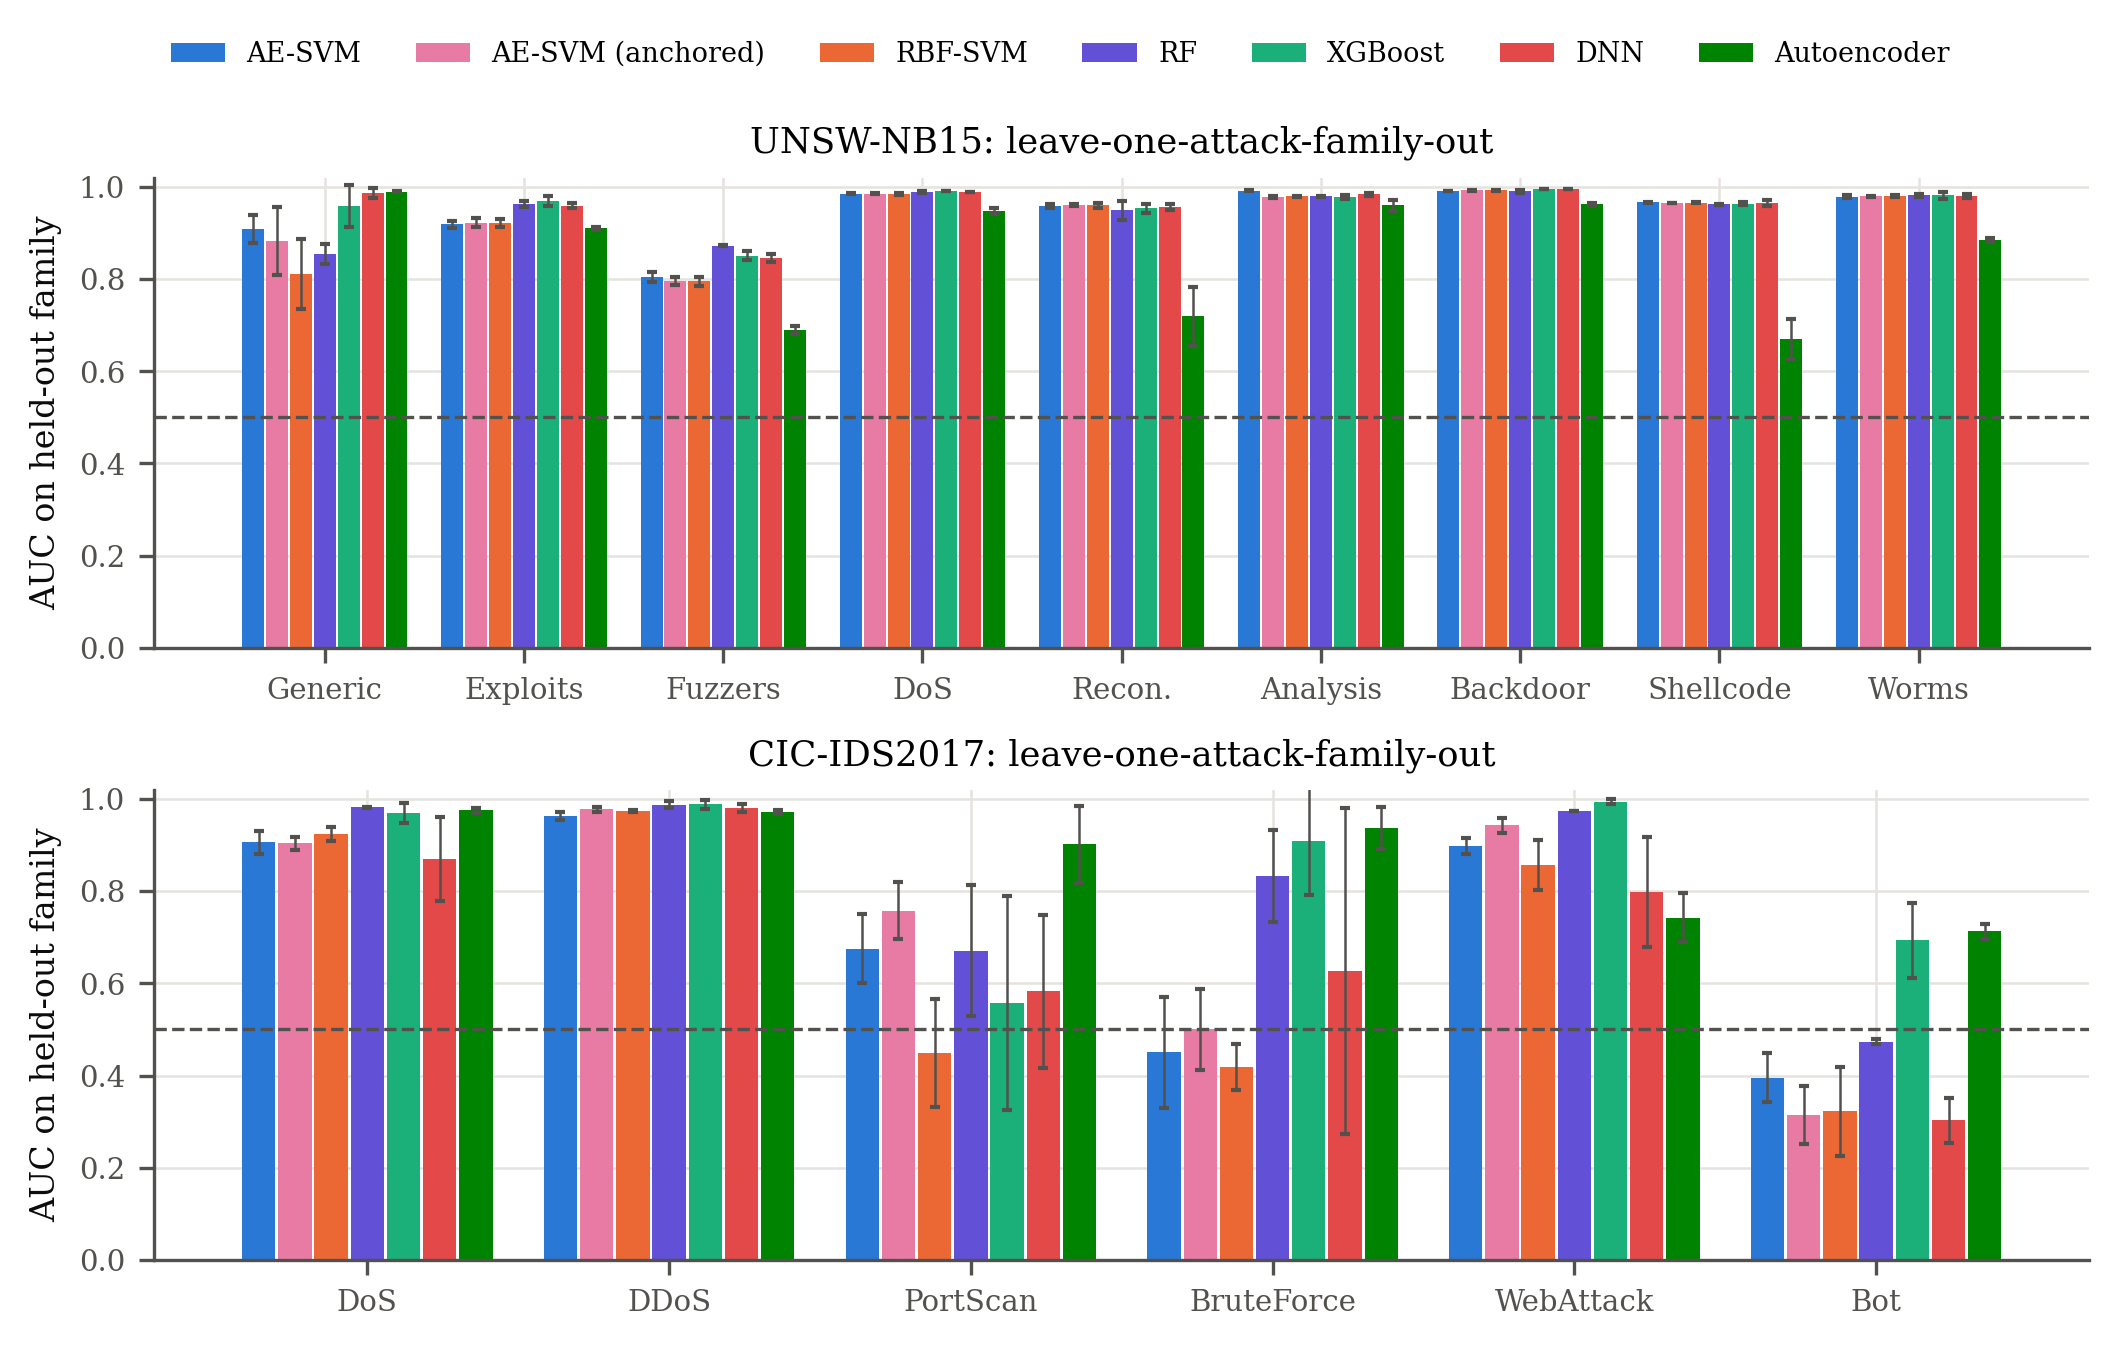
\includegraphics[width=\textwidth]{fig17_real_zeroday.png}
  \caption{Leave-one-attack-family-out ROC-AUC on the public benchmarks (mean $\pm$ 95\% CI, 3 seeds).}
  \label{fig:realzd}
\end{figure*}

@REAL_TEXT@

\section{Discussion}
\label{sec:discussion}

\subsection{Does the Amplitude-Encoding Kernel Help? A Negative Result}

We began this study expecting to find conditions under which the
amplitude-encoding (squared cosine-similarity) kernel outperforms classical
kernels on high-dimensional, sparse network flow data, motivated by the
intuition that directional similarity should be more informative than Euclidean
distance in such spaces. Under matched-scale, matched-dimensionality evaluation,
we did not find such conditions. Across training sizes $n\in\{50,\dots,5000\}$
(Fig.~\ref{fig:matched_n}) and feature dimensionalities $d\in\{16,\dots,256\}$
(Fig.~\ref{fig:dimensionality}), AE-SVM is never reliably ahead of RBF-SVM, and
is behind it at both the smallest and largest scales tested. The kernel-target
alignment analysis (Fig.~\ref{fig:alignment}) gives a mechanistic reason: on this
data, RBF's induced feature space aligns \emph{more}, not less, with the true
label structure than the amplitude-encoded one, for every attack type. The
intuition that motivated this paper---that normalizing away magnitude and
keeping only direction is a good simplification for network flow features---is
not supported by the data we generated.

We think this negative result is worth reporting for two reasons. First, our
companion study on QKD physical-layer telemetry reached the same conclusion
using the identical kernel~\cite{kapoor2026hyqad}: across two structurally
different security domains, we have not found a dataset where amplitude
encoding's cosine-similarity inductive bias earns its keep over a standard RBF
kernel. Second, ``quantum-inspired'' feature maps like amplitude encoding are
increasingly proposed for security applications on the strength of their
theoretical novelty; our results are a concrete, reproducible counter-example
that such maps should be validated empirically, under matched-scale conditions,
before being adopted -- an in-distribution accuracy gain evaluated only at one
$(n,d)$ operating point can look like a durable advantage that a matched-scale
sweep shows is not there.

\subsection{The Zero-Day Generalization Gap}

On synthetic flows, the one place plain AE-SVM and RBF-SVM diverge sharply is
generalization to unseen attack types (Fig.~\ref{fig:zeroday}), and the controls
in Section~\ref{sec:results} identify the cause: amplitude encoding discards the
input's norm, which there is the signal that separates a novel attack from
normal traffic. Our companion QKD study~\cite{kapoor2026hyqad} finds the same
mechanism when its one magnitude-carrying feature is removed. The public
benchmarks (Section~\ref{sec:real}) show that this is not a general property of
real traffic: there AE-SVM matches or slightly exceeds RBF-SVM on held-out
families. For practitioners the lesson is that a kernel's invariances predict
\emph{how} it can fail, but only a held-out-family evaluation on representative
data shows \emph{whether} it does.

\subsection{Certified Robustness: A Modest, Neutral-to-Negative Result}

The certified-robustness comparison (Table~\ref{tab:robustness}) does not show a
Lipschitz-driven advantage for amplitude encoding either: mean certified radii
are comparable between the two kernels, with RBF-SVM slightly higher and more
consistent across attack types, and AE-SVM abstaining more often. Eq.~\ref{eq:lipschitz} explains why: normalization only contracts
perturbations of large-norm inputs, and standardized benign flows cluster near
the origin, where it amplifies them; we observe no certified-radius advantage
over RBF-SVM at our certification budget ($n=300$ Monte Carlo samples).

\subsection{The One Real Advantage: Latency}

The single result in this paper that favors AE-SVM outright is inference
latency (Section~\ref{sec:latency}): the Nystr\"om-approximated AE-SVM is about
$1.2\times$ faster per sample than the equivalent RBF-SVM, because squared
cosine similarity is one normalized dot product per landmark versus RBF's
exponential. This is a genuine, mechanistically obvious advantage, but a small
one in absolute terms ($0.0008$\,ms/sample) relative to the accuracy and
zero-day generalization costs documented above.

\subsection{Limitations}

Several limitations merit acknowledgment. First, our synthetic network flow
generator (Section~\ref{sec:experiments}) is a marginal-plus-copula model, not a
packet-level simulation; the public benchmarks of Section~\ref{sec:real} address
this in part, but both have known labeling and distribution artifacts, and
neither is live zero-trust telemetry. Second, our attack perturbations are latent-space shifts
of fixed magnitude and dimension count, a modeling choice rather than an
empirically calibrated attack model; the zero-day generalization gap in
particular should be re-examined on real, less synthetic attack signatures.
Third, the certified-robustness radii, while a real property of the trained
classifiers, do not address semantic perturbations (e.g., mimicry attacks that
preserve a flow's statistical profile while changing its content), and our
certification budget ($n=300$ noise draws) leaves the achieved median radius
ceiling-saturated rather than fully resolved (Section~\ref{sec:results}).
Fourth, our deep baselines are a feed-forward DNN and a single Kitsune-style
autoencoder; graph and sequence models over flow histories may be stronger, and
kernel hyperparameters were not tuned per dataset for any kernel.

\FloatBarrier
\section{Conclusion}
\label{sec:conclusion}

Under a matched-scale, matched-dimensionality protocol, the amplitude-encoding
kernel gives no in-distribution advantage over an RBF kernel for zero-trust flow
anomaly detection, on synthetic flows or on UNSW-NB15 and CIC-IDS2017, and it
needs more data than RBF at small $n$. On synthetic flows it fails on attack
types absent from training; that failure follows from its invariance to input
norm, and appending a single norm-anchor coordinate before encoding repairs most
of it while also improving in-distribution accuracy. On UNSW-NB15 and
CIC-IDS2017 it does not fail@CONC_REAL@, which shows that held-out-attack
evaluation on real traffic, not only on a simulator, is needed before drawing
conclusions about a kernel's generalization. Our
companion QKD study~\cite{kapoor2026hyqad} finds the same mechanism in a
physical-layer domain. Quantum-inspired detectors for security should be
evaluated on unseen attack types and their invariances checked before
deployment. Natural next steps are angle and entangling feature maps, whose
invariances differ, and evaluation on live enterprise telemetry.

\section*{Code and Data Availability}
The full implementation (network flow simulator, amplitude-encoding/RBF/Laplacian/
polynomial kernel SVMs with Nystr\"om approximation, randomized-smoothing
certification, and all experiment scripts) and the result files backing every
table and figure in this paper are available at
\url{https://github.com/arnavk23/quasar-security}.

\section*{Acknowledgments}

The author thanks the IISER Bhopal Department of Computer Science for computational
resources. We thank the open-source Python ecosystem
(NumPy, SciPy, scikit-learn, XGBoost, Matplotlib) for enabling rapid prototyping of
kernel-method and quantum-inspired machine learning pipelines on commodity hardware.

\bibliographystyle{IEEEtran}
\bibliography{../references}

\end{document}
